\chapter{Heterocyclic Chemistry}\label{ch:b3:heterocycles}

A cup of coffee holds caffeine, built of two fused rings that contain four
nitrogen atoms, and its aroma comes from dozens of furans, pyrroles, pyrazines
and thiophenes formed in roasting. Most drugs on a pharmacy shelf contain at
least one ring with a nitrogen, oxygen or sulfur atom in it, and so do the bases
of DNA, \omterm{def:b3:bioinorganic:haem}{haem} and chlorophyll, and many vitamins. This chapter explains how a
heteroatom in an aromatic ring changes its electrons: it can make the ring
poorer or richer than benzene, and that decides where and how it reacts. It
ends with three classical ways of building such rings.

\begin{recall}
The Year 2 volume treated aromaticity and Hückel's rule, arenes and
electrophilic aromatic substitution through the Wheland intermediate,
activating and directing groups, amines and their basicity, imines, enamines,
tautomers and the nucleobases; the Year 1 volume $\mathrm pK_a$, nucleophiles,
electrophiles and leaving groups. \Cref{ch:b3:pericyclic} gave the [3,3]
\omterm{def:b3:pericyclic:families}{sigmatropic rearrangement}.
\end{recall}

\begin{omfigure}
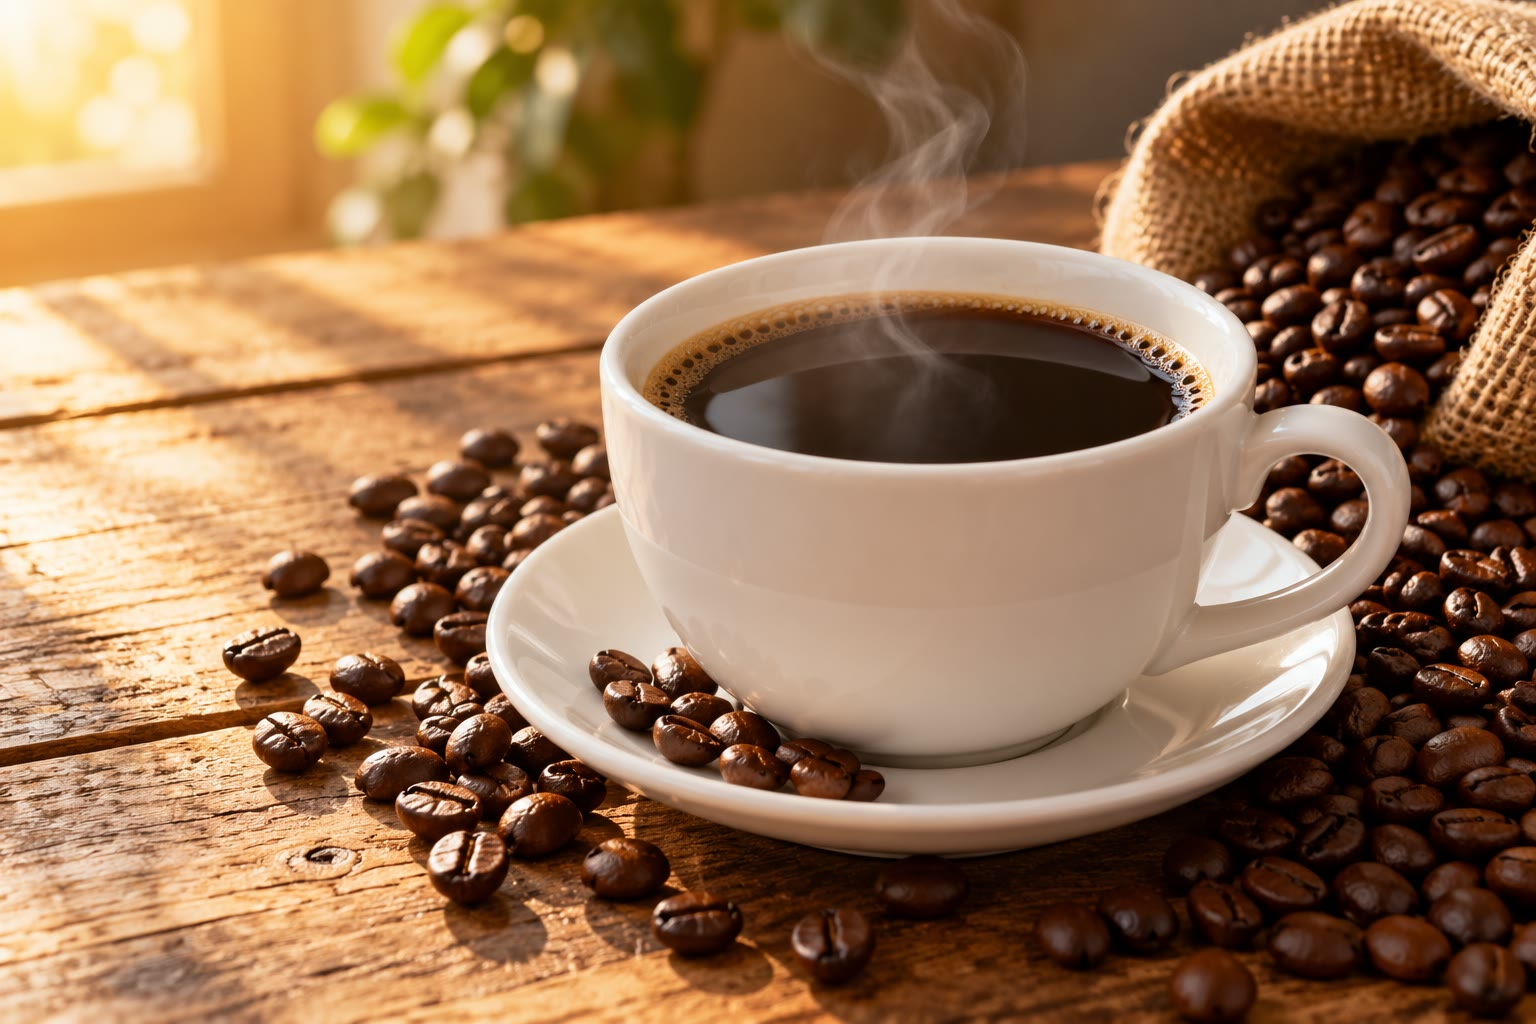
\includegraphics[width=0.5\linewidth]{images/book4/ai/b3-29-coffee.jpg}

{\small A cup of coffee and roasted beans: caffeine, a purine, and many of the
aroma molecules formed in roasting are \omterm{def:b3:heterocycles:heterocycle}{heterocycles}.}
\end{omfigure}

\section{Aromatic heterocycles}

\begin{definition}[Heterocycles]\label{def:b3:heterocycles:heterocycle}
A \emph{heterocycle}\index{heterocycle} is a ring compound with at least one
atom other than carbon in the ring; a \emph{heteroaromatic
compound}\index{heteroaromatic compound} is an aromatic one, such as pyridine,
pyrrole, furan or thiophene.
\end{definition}

\begin{proposition}[Six $\pi$ electrons]\label{prop:b3:heterocycles:sextet}
Pyridine, pyrrole, furan, thiophene and imidazole each have six $\pi$ electrons in
a planar, cyclic, conjugated ring, and are aromatic by Hückel's rule.
\end{proposition}

\begin{proof}
Pyridine: five carbons and the nitrogen each give one p electron; the nitrogen
lone pair is in an $sp^2$ orbital in the ring plane, outside the $\pi$ system: $5 + 1 = 6$.
Pyrrole: four carbons give one each and the nitrogen, bonded to H in the plane,
puts its lone pair in its p orbital: $4 + 2 = 6$. Furan and thiophene: as pyrrole, the
heteroatom giving one of its two lone pairs (the other lies in the plane). Imidazole:
the N--H nitrogen gives two, the pyridine-like nitrogen one, the three carbons
three: 6. Six is $4n + 2$ with $n = 1$.
\end{proof}

\begin{omfigure}
\begin{tikzpicture}[font=\small, yscale=0.55]
  % pyridine: six p orbitals perpendicular to the ring (drawn first), N at 0 deg
  \foreach \a in {0,60,...,300} { \pic at (\a:1.1) {omp={0.62}{90}}; }
  \draw[thick] (0:1.1) -- (60:1.1) -- (120:1.1) -- (180:1.1) -- (240:1.1) -- (300:1.1) -- cycle;
  \node[fill=white, inner sep=0.5pt] at (0:1.1) {N};
  \pic at ($(0:1.1)+(0.2,0)$) {omlobe={0.8}{0}};
  \node[font=\scriptsize, align=center, anchor=north] at (0,-2.4) {pyridine: 6 p electrons from 6 atoms;\\ lone pair in the plane (basic)};
  \begin{scope}[xshift=5.4cm]
    \foreach \a in {0,72,144,216,288} { \pic at (\a:1.0) {omp={0.62}{90}}; }
    \draw[thick] (0:1.0) -- (72:1.0) -- (144:1.0) -- (216:1.0) -- (288:1.0) -- cycle;
    \node[fill=white, inner sep=0.5pt] at (0:1.0) {N};
    \draw ($(0:1.0)+(0.18,0)$) -- (0:1.7) node[right, inner sep=0.5pt] {H};
    \node[font=\scriptsize, align=center, anchor=north] at (0,-2.4) {pyrrole: the N lone pair is one of\\ the 6 $\pi$ electrons (not basic)};
  \end{scope}
\end{tikzpicture}

{\small The $\pi$ systems of pyridine and pyrrole, seen obliquely: one p orbital per
ring atom, perpendicular to the ring. In pyridine the nitrogen lone pair (the lobe in the plane, at the
nitrogen) points outwards in the ring plane and is free to bind a proton; in pyrrole
the nitrogen, which carries a hydrogen in the plane, gives its lone pair to the
aromatic sextet.}
\end{omfigure}

\begin{definition}[$\pi$-excessive and $\pi$-deficient heterocycles]\label{def:b3:heterocycles:pi-character}
A \emph{$\pi$-excessive heterocycle}\index{$\pi$-excessive heterocycle}, such as
pyrrole, furan or thiophene, has six $\pi$ electrons on five atoms and a higher
$\pi$ \omterm{def:b3:computational-chemistry:dft}{electron density} on its carbons than benzene; a \emph{$\pi$-deficient
heterocycle}\index{$\pi$-deficient heterocycle}, such as pyridine, has an
electronegative ring atom that draws $\pi$ density away from the carbons.
\end{definition}

\begin{proposition}[Basicity]\label{prop:b3:heterocycles:basicity}
Pyridine is a moderate base and pyrrole almost none; pyrrole, when it is
protonated in strong acid, takes the proton on carbon, not nitrogen.
\end{proposition}

\begin{proof}[Argued]
% ledger: pka:pyridinium, pka4:pyrrolium, pka4:piperidinium, pka4:imidazolium, pka4:DMAPH
Pyridine's lone pair is outside the $\pi$ system: protonating it costs no
aromaticity, and pyridinium has $\mathrm pK_a = 5.2$; it is less basic than piperidine
(pyridinium's nitrogen is $sp^2$, with more s character, and holds its pair more
tightly: piperidinium 11.1). Protonating pyrrole's nitrogen would take its lone
pair out of the sextet and destroy the aromaticity; only very strong acids
protonate pyrrole at all, at C2, where the cation keeps some delocalisation
($\mathrm pK_a$ about $-4$). Imidazole has both kinds of nitrogen: it is protonated on the
pyridine-like one, and its cation, symmetrical, is stabilised by resonance ($\mathrm pK_a$
7.0), the reason histidine works as an acid and a base in \omterm{def:b3:complex-kinetics:enzyme}{enzymes}.
4-(Dimethylamino)pyridine is more basic still ($\mathrm pK_a$ 9.6): the amino group pushes
its lone pair into the ring and onto the ring nitrogen.
\end{proof}

% ledger: dip:pyridine, dip4:pyrrole, dip4:furan, dip4:thiophene
The dipole moments tell the same story: pyridine (\qty{2.19}{D}) has its negative end
on nitrogen, while in pyrrole (\qty{1.84}{D}) the donation of the lone pair to the ring
puts the negative end on the ring and the positive end on nitrogen. In furan
(\qty{0.66}{D}) and thiophene (\qty{0.55}{D}) the two effects, $\sigma$ withdrawal and $\pi$ donation, nearly
cancel.

\begin{omfigure}
% ledger: h1:pyridine.a, h1:pyridine.g, h1:pyridine.b, h1:pyrrole.a, h1:pyrrole.b, h1:pyrrole.NH, h1:furan.a, h1:furan.b
\begin{tikzpicture}
\begin{axis}[width=0.86\linewidth, height=6.2cm, x dir=reverse, xmin=5.8, xmax=9.0, ymin=-0.1, ymax=3.6,
  axis x line=bottom, axis y line=none, xlabel={$\delta$ / ppm}, tick label style={font=\scriptsize}, label style={font=\small}]
\addplot[omDef, thick] table[x=ppm, y expr=\thisrow{y}+2.4] {figdata/out/bachelor-3-heterocycle-nmr-pyridine.dat};
\addplot[omThm, thick] table[x=ppm, y expr=\thisrow{y}+1.2] {figdata/out/bachelor-3-heterocycle-nmr-pyrrole.dat};
\addplot[omMeth, thick] table[x=ppm, y=y] {figdata/out/bachelor-3-heterocycle-nmr-furan.dat};
\node[font=\scriptsize, omDef, anchor=west] at (axis cs:7.1,3.0) {pyridine: H2/6, H4, H3/5 (2\,:\,1\,:\,2)};
\node[font=\scriptsize, omThm, anchor=west] at (axis cs:7.7,1.8) {pyrrole: NH, H2/5, H3/4};
\node[font=\scriptsize, omMeth, anchor=west] at (axis cs:7.2,0.6) {furan: H2/5, H3/4};
\end{axis}
\end{tikzpicture}

{\small Proton NMR of pyridine, pyrrole and furan in deuterochloroform,
synthesised from measured shifts as single lines (couplings omitted), with
areas equal to the numbers of protons. The $\pi$-deficient pyridine has its H2/6 and H4
signals well downfield of benzene's; the $\pi$-excessive pyrrole and furan have most
of theirs upfield of it; the protons next to the heteroatom are always the most
deshielded.}
\end{omfigure}

\section{Pyridine}

Pyridine resists electrophilic substitution: the electrophile meets a ring
poorer in electrons than benzene, and, in the acid usually present, a
pyridinium ion whose positive charge repels it. Nitration needs very forcing
conditions and gives the 3-isomer in poor yield.

\begin{proposition}[Electrophilic substitution at C3]\label{prop:b3:heterocycles:pyridine-c3}
Electrophilic attack on pyridine occurs at C3: attack at C2 or C4 gives a
Wheland intermediate one of whose resonance structures puts the positive
charge on nitrogen with only six electrons around it.
\end{proposition}

\begin{proof}
In the cation from attack at C2 (or C4) the positive charge is spread over C3, C5
and N1 (or C3, C5 and N1): a resonance structure with an electron-deficient,
six-electron nitrogen, very unfavourable for an electronegative atom. Attack
at C3 spreads the charge over C2, C4 and C6 only. All three cations are less stable
than benzene's, but C3 attack is the least bad.
\end{proof}

\begin{definition}[Pyridine N-oxide]\label{def:b3:heterocycles:n-oxide}
A \emph{pyridine N-oxide}\index{pyridine N-oxide}, made by oxidising pyridine
with a peroxy acid, has an $\mathrm{N^+{-}O^-}$ group whose oxygen gives electrons back to C2
and C4; it undergoes electrophilic substitution at C4, and the oxygen is then
removed.
\end{definition}

\begin{definition}[Nucleophilic aromatic substitution]\label{def:b3:heterocycles:snar}
\emph{Nucleophilic aromatic substitution}\index{nucleophilic aromatic substitution}
($\mathrm S_\mathrm NAr$) replaces a leaving group on an electron-poor aromatic ring
by a nucleophile, through addition followed by elimination. The anionic
addition intermediate is a \emph{Meisenheimer complex}\index{Meisenheimer complex}.
\end{definition}

\begin{proposition}[$\mathrm S_\mathrm NAr$ at C2 and C4]\label{prop:b3:heterocycles:snar-positions}
Halopyridines undergo $\mathrm S_\mathrm NAr$ readily at C2 and C4 and only sluggishly at C3,
because addition at C2 or C4 places the negative charge on the nitrogen.
\end{proposition}

\begin{proof}
Addition at C2 makes C2 $sp^3$ and leaves four $\pi$ electrons plus the incoming pair
spread over N1, C3 and C5 (or for C4: C3, C5 and N1): one resonance structure has the
negative charge on the electronegative nitrogen. Addition at C3 spreads it over
C2, C4 and C6 only, all carbons.
\end{proof}

\begin{omfigure}
\begin{tikzpicture}[font=\small, >=Stealth]
  \draw[thick] (-0.000,-0.620) -- (0.537,-0.310) -- (0.537,0.310) -- (0.000,0.620) -- (-0.537,0.310) -- (-0.537,-0.310) -- cycle;
  \draw[thick] (0.082,-0.424) -- (0.326,-0.283);
  \draw[thick] (0.326,0.283) -- (0.082,0.424);
  \draw[thick] (-0.408,0.141) -- (-0.408,-0.141);
  \node[fill=white, inner sep=0.4pt, font=\scriptsize] at (-0.000,-0.620) {N};
  \draw (0.537,-0.310) -- (0.927,-0.535) node[right, inner sep=0.5pt, font=\scriptsize] {Cl};
  \draw[thick] (3.400,-0.620) -- (3.937,-0.310) -- (3.937,0.310) -- (3.400,0.620) -- (2.863,0.310) -- (2.863,-0.310) -- cycle;
  \draw[thick] (3.726,0.283) -- (3.482,0.424);
  \draw[thick] (2.992,0.141) -- (2.992,-0.141);
  \node[fill=white, inner sep=0.4pt, font=\scriptsize] at (3.400,-0.620) {N};
  \node[font=\scriptsize, omThm] at (3.350,-0.920) {$\ominus$};
  \draw (3.937,-0.310) -- (4.386,-0.343) node[right, inner sep=0.5pt, font=\scriptsize] {Nu};
  \draw (3.937,-0.310) -- (4.190,-0.682) node[right, inner sep=0.5pt, font=\scriptsize] {Cl};
  \draw[thick] (6.800,-0.620) -- (7.337,-0.310) -- (7.337,0.310) -- (6.800,0.620) -- (6.263,0.310) -- (6.263,-0.310) -- cycle;
  \draw[thick] (6.882,-0.424) -- (7.126,-0.283);
  \draw[thick] (7.126,0.283) -- (6.882,0.424);
  \draw[thick] (6.392,0.141) -- (6.392,-0.141);
  \node[fill=white, inner sep=0.4pt, font=\scriptsize] at (6.800,-0.620) {N};
  \draw (7.337,-0.310) -- (7.727,-0.535) node[right, inner sep=0.5pt, font=\scriptsize] {Nu};
  \draw[->, thick] (1.25,0) -- (2.35,0) node[midway, above, font=\scriptsize] {$+\,\mathrm{Nu^-}$};
  \draw[->, thick] (4.65,0) -- (5.75,0) node[midway, above, font=\scriptsize] {$-\,\ce{Cl-}$};
  \node[font=\scriptsize] at (3.4,-1.2) {Meisenheimer complex};
\end{tikzpicture}

{\small Nucleophilic substitution of 2-chloropyridine: the nucleophile adds to
C2, giving an anionic intermediate whose negative charge sits largely on the
ring nitrogen (one resonance structure shown); chloride then leaves and the
aromatic ring is restored.}
\end{omfigure}

\begin{proposition}[Addition--elimination]\label{prop:b3:heterocycles:snar-mechanism}
For an $\mathrm S_\mathrm NAr$ reaction whose addition step is rate-determining, $v = k[\mathrm{ArX}][\mathrm{Nu^-}]$,
and fluoride is the best halide leaving group.
\end{proposition}

\begin{proof}[Argued]
The rate is that of the bimolecular addition. The carbon--halogen bond is not
broken in that step; what matters is how much the halogen lowers the energy of
the anionic transition state by withdrawing electrons, and fluorine, the most
electronegative, does so most: the order F $>$ Cl $\approx$ Br $>$ I, opposite to that of $\mathrm S_\mathrm N2$.
\end{proof}

\begin{definition}[Chichibabin reaction]\label{def:b3:heterocycles:chichibabin}
The \emph{Chichibabin reaction}\index{Chichibabin reaction} is the amination of
pyridine at C2 by sodium amide: the amide ion adds to C2, and a hydride ion is
lost, as dihydrogen after reaction with the product.
\end{definition}

Pyridine and DMAP also serve as bases and as nucleophilic catalysts: in
acylations with acid anhydrides, DMAP attacks the anhydride first, giving an
acylpyridinium ion that transfers its acyl group to the alcohol much faster than
the anhydride itself. Pyridines, bipyridines and phenanthrolines are among the
commonest ligands of coordination chemistry.

\section{Five-membered rings}

\begin{proposition}[Electrophilic substitution of pyrrole at C2]\label{prop:b3:heterocycles:pyrrole-c2}
Pyrrole, furan and thiophene undergo electrophilic substitution mainly at C2,
because the cation from attack at C2 has three resonance structures and that
from attack at C3 only two.
\end{proposition}

\begin{proof}
After attack at C2, the positive charge can sit on C3, on C5, or on nitrogen,
where it is shared through the lone pair and every atom keeps an octet (third
structure). After attack at C3, it can sit on C2 or on nitrogen only: the charge
is less delocalised (see the figure).
\end{proof}

\begin{omfigure}
\begin{tikzpicture}[font=\small]
  \draw[thick] (0.000,0.620) -- (0.590,0.192) -- (0.364,-0.502) -- (-0.364,-0.502) -- (-0.590,0.192) -- cycle;
  \draw[thick] (-0.303,-0.269) -- (-0.403,0.039);
  \node[fill=white, inner sep=0.4pt, font=\scriptsize] at (0.000,0.620) {N};
  \draw (0.000,0.750) -- (0.000,1.020) node[above, inner sep=0.5pt, font=\scriptsize] {H};
  \draw (0.590,0.192) -- (0.893,0.482) node[right, inner sep=0.5pt, font=\scriptsize] {H};
  \draw (0.590,0.192) -- (1.006,0.135) node[right, inner sep=0.5pt, font=\scriptsize] {E};
  \node[font=\scriptsize, omThm] at (0.164,-0.226) {$\oplus$};
  \draw[thick] (2.600,0.620) -- (3.190,0.192) -- (2.964,-0.502) -- (2.236,-0.502) -- (2.010,0.192) -- cycle;
  \draw[thick] (2.762,-0.371) -- (2.438,-0.371);
  \node[fill=white, inner sep=0.4pt, font=\scriptsize] at (2.600,0.620) {N};
  \draw (2.600,0.750) -- (2.600,1.020) node[above, inner sep=0.5pt, font=\scriptsize] {H};
  \draw (3.190,0.192) -- (3.493,0.482) node[right, inner sep=0.5pt, font=\scriptsize] {H};
  \draw (3.190,0.192) -- (3.606,0.135) node[right, inner sep=0.5pt, font=\scriptsize] {E};
  \node[font=\scriptsize, omThm] at (2.335,0.086) {$\oplus$};
  \draw[thick] (5.200,0.620) -- (5.790,0.192) -- (5.564,-0.502) -- (4.836,-0.502) -- (4.610,0.192) -- cycle;
  \draw[thick] (5.362,-0.371) -- (5.038,-0.371);
  \draw[thick] (5.113,0.395) -- (4.851,0.205);
  \node[fill=white, inner sep=0.4pt, font=\scriptsize] at (5.200,0.620) {N};
  \draw (5.200,0.750) -- (5.200,1.020) node[above, inner sep=0.5pt, font=\scriptsize] {H};
  \draw (5.790,0.192) -- (6.093,0.482) node[right, inner sep=0.5pt, font=\scriptsize] {H};
  \draw (5.790,0.192) -- (6.206,0.135) node[right, inner sep=0.5pt, font=\scriptsize] {E};
  \node[font=\scriptsize, omThm] at (5.480,0.700) {$\oplus$};
  \draw[thick] (8.400,0.620) -- (8.990,0.192) -- (8.764,-0.502) -- (8.036,-0.502) -- (7.810,0.192) -- cycle;
  \draw[thick] (8.097,-0.269) -- (7.997,0.039);
  \node[fill=white, inner sep=0.4pt, font=\scriptsize] at (8.400,0.620) {N};
  \draw (8.400,0.750) -- (8.400,1.020) node[above, inner sep=0.5pt, font=\scriptsize] {H};
  \draw (8.764,-0.502) -- (9.135,-0.700) node[right, inner sep=0.5pt, font=\scriptsize] {H};
  \draw (8.764,-0.502) -- (8.839,-0.915) node[right, inner sep=0.5pt, font=\scriptsize] {E};
  \node[font=\scriptsize, omThm] at (8.665,0.086) {$\oplus$};
  \draw[thick] (11.000,0.620) -- (11.590,0.192) -- (11.364,-0.502) -- (10.636,-0.502) -- (10.410,0.192) -- cycle;
  \draw[thick] (10.697,-0.269) -- (10.597,0.039);
  \draw[thick] (11.087,0.395) -- (11.349,0.205);
  \node[fill=white, inner sep=0.4pt, font=\scriptsize] at (11.000,0.620) {N};
  \draw (11.000,0.750) -- (11.000,1.020) node[above, inner sep=0.5pt, font=\scriptsize] {H};
  \draw (11.364,-0.502) -- (11.735,-0.700) node[right, inner sep=0.5pt, font=\scriptsize] {H};
  \draw (11.364,-0.502) -- (11.439,-0.915) node[right, inner sep=0.5pt, font=\scriptsize] {E};
  \node[font=\scriptsize, omThm] at (11.280,0.700) {$\oplus$};
  \node[font=\scriptsize] at (2.6,-1.35) {attack at C2: three structures};
  \node[font=\scriptsize] at (9.7,-1.35) {attack at C3: two structures};
  \draw[black!40] (6.8,-1.2) -- (6.8,1.2);
\end{tikzpicture}

{\small Wheland intermediates of pyrrole (E: the electrophile; $\oplus$: positive charge).
Attack at C2 gives a cation with the charge on C3, on C5, or on the nitrogen with all
octets complete; attack at C3, on C2 or nitrogen only.}
\end{omfigure}

Pyrrole is about as reactive as phenol or aniline: it is brominated, nitrated
and acylated under mild conditions, polymerises in strong acid, and is
formylated at C2 by the Vilsmeier reagent from dimethylformamide and phosphoryl
chloride. Reactivities fall in the order pyrrole $>$ furan $>$ thiophene $>$ benzene,
following the willingness of the heteroatom to share its lone pair. Furan,
the least aromatic, also reacts as a diene in Diels--Alder reactions. Strong
bases such as butyllithium deprotonate furan and thiophene at C2, next to the
heteroatom, giving organolithium reagents.

\begin{method}[Predicting the site of attack on a heterocycle]\label{met:b3:heterocycles:site}
\begin{enumerate}
  \item Classify the ring: $\pi$-excessive (pyrrole-like heteroatom) or $\pi$-deficient
        (pyridine-like nitrogen).
  \item Electrophiles: on a $\pi$-excessive ring at C2 (C3 for indole, whose C2 attack
        would disrupt the benzene ring); on pyridine at C3, or at C4 through the
        N-oxide.
  \item Nucleophiles: on a $\pi$-deficient ring at C2 or C4, especially with a leaving
        group there.
  \item Strong bases: at the C--H next to the heteroatom.
\end{enumerate}
\end{method}

\section{Fused and biological heterocycles}

Indole, a benzene fused to a pyrrole, reacts with electrophiles at C3: there the
intermediate keeps the benzene ring intact, with the charge on the nitrogen.
Quinoline, a benzene fused to a pyridine, is substituted by electrophiles on
its benzene ring and by nucleophiles at C2 and C4. The nucleobases are
pyrimidines (cytosine, thymine, uracil) and purines (adenine, guanine), a
pyrimidine fused to an imidazole. Their oxo and amino forms (lactam and amine
tautomers) dominate over the hydroxy and imino forms, which fixes the pattern of
hydrogen-bond donors and acceptors on each base, and so the base pairing.

\begin{omfigure}
\begin{tikzpicture}[font=\small]
  \node[draw, rounded corners, minimum width=1.8cm, minimum height=2.8cm, fill=omDef!8] at (0,0) {};
  \node[font=\small\bfseries] at (0,1.75) {guanine};
  \node[anchor=east] (g1) at (0.85,0.85) {C6=O};
  \node[anchor=east] (g2) at (0.85,0) {N1--H};
  \node[anchor=east] (g3) at (0.85,-0.85) {C2--N--H};
  \node[draw, rounded corners, minimum width=1.8cm, minimum height=2.8cm, fill=omThm!8] at (3.2,0) {};
  \node[font=\small\bfseries] at (3.2,1.75) {cytosine};
  \node[anchor=west] (c1) at (2.35,0.85) {H--N--C4};
  \node[anchor=west] (c2) at (2.35,0) {N3};
  \node[anchor=west] (c3) at (2.35,-0.85) {O=C2};
  \draw[omMeth, very thick, dotted] (g1.east) -- (c1.west);
  \draw[omMeth, very thick, dotted] (g2.east) -- (c2.west);
  \draw[omMeth, very thick, dotted] (g3.east) -- (c3.west);
\end{tikzpicture}

{\small A guanine--cytosine base pair, schematic: three hydrogen bonds (green)
between the carbonyl oxygen of guanine and an amino N--H of cytosine, the N1--H of
guanine and the ring N3 of cytosine, and an amino N--H of guanine and the
carbonyl oxygen of cytosine. Adenine and thymine form two.}
\end{omfigure}

\section{Making rings}

\begin{definition}[Paal--Knorr synthesis]\label{def:b3:heterocycles:paal-knorr}
The \emph{Paal--Knorr synthesis}\index{Paal--Knorr synthesis} makes a furan
(with acid), a pyrrole (with a primary amine or ammonia) or a thiophene (with a
sulfur reagent) from a 1,4-dicarbonyl compound.
\end{definition}

\begin{definition}[Hantzsch pyridine synthesis]\label{def:b3:heterocycles:hantzsch}
The \emph{Hantzsch pyridine synthesis}\index{Hantzsch pyridine synthesis}
condenses an aldehyde, two equivalents of a $\beta$-keto ester and ammonia into a
1,4-dihydropyridine, which can be oxidised to the pyridine.
\end{definition}

\begin{definition}[Fischer indole synthesis]\label{def:b3:heterocycles:fischer-indole}
The \emph{Fischer indole synthesis}\index{Fischer indole synthesis} heats the
phenylhydrazone of an aldehyde or ketone with an acid catalyst: the hydrazone
tautomerises to an ene-hydrazine, which undergoes a [3,3] \omterm{def:b3:pericyclic:families}{sigmatropic
rearrangement}; cyclisation and loss of ammonia give the indole.
\end{definition}

\begin{omfigure}
\setchemfig{atom sep=1.8em}
\schemestart
\chemfig{*6(-=-=(-NH-[:30]N=[:-30](-[:-90]CH_3)-[:30]CH_3)-=)}
\arrow{->[$\ce{H+}$][tautomer]}[,1.4]
\chemfig{*6(-=-=(-NH-[:30]NH-[:-30](=[:-90]CH_2)-[:30]CH_3)-=)}
\schemestop
\par\bigskip
\schemestart
\arrow{->[{[3,3]}, then][cyclisation, $-\ce{NH3}$]}[,2.2]
\chemfig{*6(-=*5(-=(-CH_3)-N(-H)-)-=-=)}
\schemestop

{\small The \omterm{def:b3:heterocycles:fischer-indole}{Fischer indole synthesis} from acetone phenylhydrazone. Acid turns the
hydrazone into its ene-hydrazine tautomer; the [3,3] rearrangement breaks the
N--N bond and makes a C--C bond between the ring carbon \textit{ortho} to nitrogen and the
terminal $\ce{CH2}$; the new amine attacks the imine, and loss of ammonia gives
2-methylindole.}
\end{omfigure}

\begin{method}[Disconnecting a heterocycle]\label{met:b3:heterocycles:disconnect}
\begin{enumerate}
  \item A 2,5-disubstituted pyrrole, furan or thiophene: disconnect both bonds to
        the heteroatom, back to a 1,4-diketone (Paal--Knorr).
  \item A symmetrical 1,4-dihydropyridine with esters at C3 and C5: back to one
        aldehyde, two $\beta$-keto esters and ammonia (Hantzsch).
  \item A 2,3-disubstituted indole: back to phenylhydrazine and the ketone
        $\mathrm{R^2CH_2COR^3}$ (Fischer).
  \item Check the availability of the pieces, then the regiochemistry when the ketone
        is unsymmetrical.
\end{enumerate}
\end{method}

\begin{definition}[Bioisostere]\label{def:b3:heterocycles:bioisostere}
A \emph{bioisostere}\index{bioisostere} is a group that replaces another in a
drug molecule while keeping its biological activity, because it has a similar
size, shape and pattern of hydrogen-bonding and charge, such as a tetrazole in
place of a carboxylic acid, or a pyridine in place of a benzene ring.
\end{definition}

\begin{inthelab}[A Paal--Knorr pyrrole]
Hexane-2,5-dione, aniline and a catalytic amount of 4-toluenesulfonic acid are
heated under reflux in toluene in a flask fitted with a Dean--Stark trap: the
water formed is carried over as an azeotrope and collects in the side arm, which
drives the condensation to completion. When no more water separates, the
solution is washed with aqueous sodium hydrogencarbonate, dried and evaporated,
and the 2,5-dimethyl-1-phenylpyrrole is recrystallised.
\end{inthelab}

\begin{safety}{\ghs[0.62cm]{GHS02}\ghs[0.62cm]{GHS06}\ghs[0.62cm]{GHS07}\ghs[0.62cm]{GHS08}\ghs[0.62cm]{GHS09}}
% ledger: ghs4:pyridine, ghs4:phenylhydrazine
Pyridine: highly flammable, harmful by all routes, with a strong smell; used in a
fume hood. Phenylhydrazine: toxic by all routes, may cause cancer and genetic
defects, damages the blood on repeated exposure, sensitising, very toxic to
aquatic life; it is weighed in a fume hood with gloves, and its waste collected
separately.
\end{safety}

\begin{history}[Two classical ring syntheses]
Emil Fischer described his indole synthesis in 1883, in the same years as his
work on the sugars and the purines; Arthur Hantzsch published his pyridine
synthesis in 1881. Both remain in use: the Fischer synthesis for the
triptan drugs against migraine, the Hantzsch synthesis for the dihydropyridine
calcium-channel blockers that treat high blood pressure.
\end{history}

\section{Exercises}

\begin{exercise}[$\star$]\label{exo:b3:heterocycles:1}
Count the $\pi$ electrons of oxazole, thiazole, pyrimidine and purine, and say which
lone pairs belong to the $\pi$ system.
\end{exercise}

\begin{exercise}[$\star$]\label{exo:b3:heterocycles:2}
Rank pyridine, pyrrole, imidazole, piperidine and DMAP by basicity, with their
$\mathrm pK_a$ values.
\end{exercise}

\begin{exercise}[$\star$]\label{exo:b3:heterocycles:3}
Give the main product of monobromination of pyrrole, of furan and of indole.
\end{exercise}

\begin{exercise}[$\star$]\label{exo:b3:heterocycles:4}
Give the products of the Paal--Knorr reaction of hexane-2,5-dione with acid alone,
with methylamine, and with phosphorus pentasulfide.
\end{exercise}

\begin{exercise}[$\star\star$]\label{exo:b3:heterocycles:5}
2-Chloropyridine reacts with sodium methoxide in methanol at \qty{65}{\celsius}; 3-chloropyridine
hardly does. Explain, and give the product.
\end{exercise}

\begin{exercise}[$\star\star$]\label{exo:b3:heterocycles:6}
Give the product of the \omterm{def:b3:heterocycles:chichibabin}{Chichibabin reaction} of pyridine and draw the addition
intermediate.
\end{exercise}

\begin{exercise}[$\star\star$]\label{exo:b3:heterocycles:7}
\omterm{def:b3:heterocycles:n-oxide}{Pyridine N-oxide} is nitrated at C4. Explain with resonance structures, and say how
4-nitropyridine is obtained.
\end{exercise}

\begin{exercise}[$\star\star$]\label{exo:b3:heterocycles:8}
2-Hydroxypyridine exists mainly as 2-pyridone in water. Draw both tautomers and
explain why the pyridone is still aromatic.
\end{exercise}

\begin{exercise}[$\star\star$]\label{exo:b3:heterocycles:9}
Give the components of a Hantzsch synthesis of the 1,4-dihydropyridine with
methyl esters at C3 and C5, methyl groups at C2 and C6 and a 2-nitrophenyl group
at C4.
\end{exercise}

\begin{exercise}[$\star\star\star$]\label{exo:b3:heterocycles:10}
Butanone gives two different indoles in the Fischer synthesis with
phenylhydrazine. Give both, and say how the acid strength changes their ratio.
\end{exercise}

\begin{exercise}[$\star\star\star$]\label{exo:b3:heterocycles:11}
Explain why 4-fluoronitrobenzene and 2-fluoropyridine react faster with
nucleophiles than the corresponding chlorides, unlike $\mathrm S_\mathrm N2$ substrates.
\end{exercise}

\begin{exercise}[$\star\star\star$]\label{exo:b3:heterocycles:12}
Using the synthetic spectra of the chapter, explain how you would tell pyridine,
pyrrole and furan apart by their proton NMR, and predict the spectrum of
thiophene (shifts \qty{7.33}{ppm} and \qty{7.12}{ppm}).
\end{exercise}

\section{Problem: Building an Indole}

\begin{problem}[{Weekend problem --- building an indole: the phenylhydrazone of
acetone, the ene-hydrazine and its [3,3] rearrangement, the loss of ammonia,
and the choice between two indoles with butanone}]
\label{pb:b3:heterocycles:1}
% ledger: aw:C, aw:H, aw:N, aw:O
Data of the problem: 10.0 g of phenylhydrazine reacts with excess acetone, and
the hydrazone is heated with zinc chloride.

\medskip\noindent\textbf{Part I --- The hydrazone.}
\begin{enumerate}
  \item Write the formation of acetone phenylhydrazone.
  \item Why is it an imine-type condensation, and why is a trace of acid useful?
  \item Which nitrogen of phenylhydrazine attacks the carbonyl group, and why?
  \item Compute the molar mass of phenylhydrazine and the amount used.
  \item Compute the theoretical mass of hydrazone.
\end{enumerate}

\medskip\noindent\textbf{Part II --- The ene-hydrazine and the [3,3] step.}
\begin{enumerate}[resume]
  \item Draw the ene-hydrazine tautomer.
  \item Which six atoms form the cyclic transition state of the [3,3] rearrangement?
  \item Which bond breaks and which forms?
  \item How many electrons take part, and is the step thermally allowed?
  \item What does the zinc chloride do?
  \item Why does the aromaticity of the benzene ring have to be restored afterwards?
\end{enumerate}

\medskip\noindent\textbf{Part III --- Closing the ring.}
\begin{enumerate}[resume]
  \item Which amine attacks which carbon to close the five-membered ring?
  \item What small molecule leaves, and what drives the last step?
  \item Write the overall equation, hydrazone to 2-methylindole.
  \item Compute the molar mass of 2-methylindole.
  \item Compute the theoretical mass of 2-methylindole.
  \item Where would 2-methylindole be substituted by an electrophile, and why?
\end{enumerate}

\medskip\noindent\textbf{Part IV --- Butanone.}
\begin{enumerate}[resume]
  \item Draw the two ene-hydrazines of butanone phenylhydrazone.
  \item Give the two indoles they lead to.
  \item Which ene-hydrazine is more substituted, and which forms under strong acid?
  \item Which indole dominates with a weak acid, and why?
  \item Why can acetaldehyde phenylhydrazone not give indole itself well?
  \item What does the regiochemistry problem mean for the synthesis of a drug?
  \item State the result: the theoretical mass of 2-methylindole from 10.0 g of
        phenylhydrazine.
\end{enumerate}
\end{problem}
